\documentclass[12pt]{article}
\PassOptionsToPackage{pdftex}{graphicx}
	\usepackage{graphicx} 

\begin{document}


\begin{figure}[tbh]
  \centering
  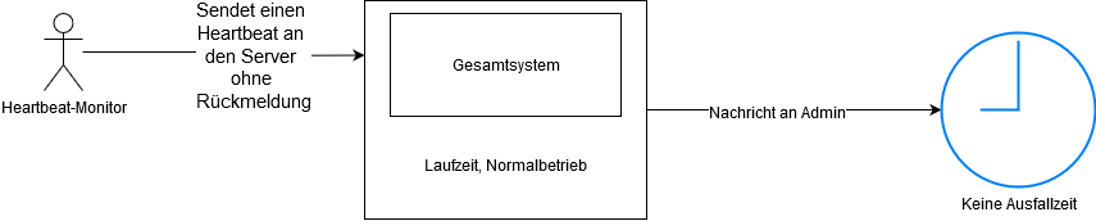
\includegraphics[width=0.7\textwidth]{Bilder/Verfuegbarkeit.png}
  \caption{Verfuegbarkeits-Szenario}
  \label{fig:Qualitaet1}
\end{figure}

Verfuegbarkeits-Szenario
Source of Stimulus: Heartbeat Monitor
Stimulus: Sendet einen Heartbeat an den Server ohne Rückmeldung
Environment: Laufzeit, Normalbetrieb
Component: Gesamtsystem
Response: Nachricht an Admin
Response Measure: …




\begin{figure}[tbh]
  \centering
  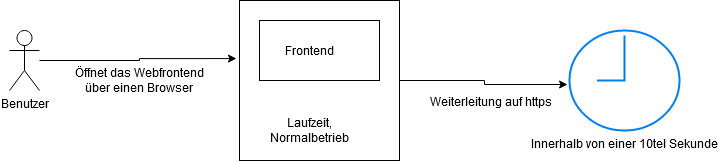
\includegraphics[width=0.7\textwidth]{Bilder/Sicherheit.png}
  \caption{Effizienz-Szenario}
  \label{fig:Qualitaet2}
\end{figure}


Sicherheits-Szenario
Source of Stimulus: Benutzer
Stimulus: Öffnet das Webfrontend über einen Browser über http
Environment: Laufzeit, Normalbetrieb
Component: Frontend
Response: Weiterleitung auf https
Response Measure: Innerhalb von einer 10tel Sekunde




\begin{figure}[tbh]
  \centering
  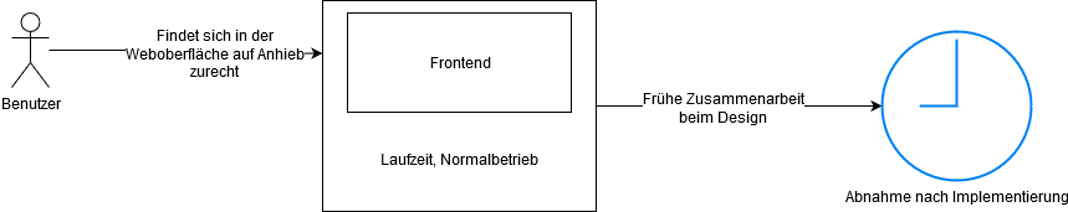
\includegraphics[width=0.7\textwidth]{Bilder/Nutzbarkeit.png}
  \caption{Nutzbarkeit-Szenario}
  \label{fig:Qualitaet3}
\end{figure}



Nutzbarkeits-Szenario
Source of Stimulus: Benutzer
Stimulus: Findet sich in der Weboberfläche auf Anhieb zurecht
Environment: Laufzeit, Normalbetrieb
Component: Frontend
Response: Frühe Zusammenarbeit beim Design
Response Measure: Abnahme nach Implementierung





\begin{figure}[tbh]
  \centering
  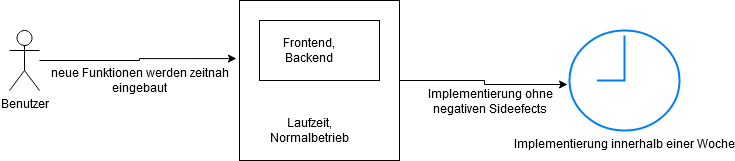
\includegraphics[width=0.7\textwidth]{Bilder/Erweiterbarkeit.png}
  \caption{Effizienz-Szenario}
  \label{fig:Qualitaet3}
\end{figure}


Erweiterbarkeits-Szenario
Source of Stimulus: Benutzer
Stimulus: Neue Funktionen werden zeitnah eingebaut
Environment: Laufzeit, Normalbetrieb
Component: Frontend, Backend
Response: Implementierung ohne negativen Sideeffects
Response Measure: Implementierung innerhalb einer Woche 



\begin{figure}[tbh]
  \centering
  \includegraphics[width=0.7\textwidth]{Bilder/Portierbarkeits.png}
  \caption{Effizienz-Szenario}
  \label{fig:Qualitaet4}
\end{figure}



Portierbarkeits-Szenario
Source of Stimulus: IT-Abteilung
Stimulus: Ein Hardwarewechsel auf eine andere Plattform
Environment: Laufzeit, Normalbetrieb
Component: Frontend, Backend
Response: Implementierung in hardwarenaher Sprache mit Compilern, die Programme für alle Systeme kompilieren 
Response Measure: Compileroutput muss auf ARM-Cortex 7, Intel x86/x64 unter Linux und Windows funktionieren




\begin{figure}[tbh]
  \centering
  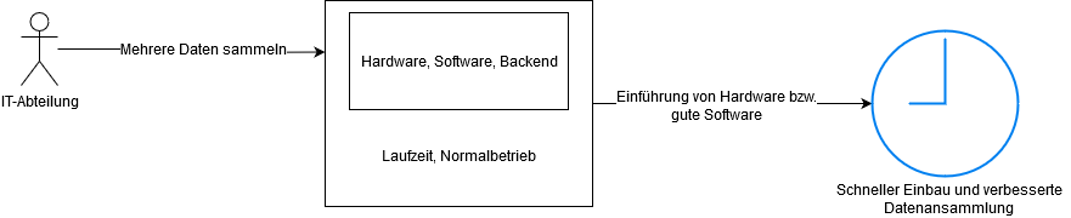
\includegraphics[width=0.7\textwidth]{Bilder/Effizienz.png}
  \caption{Effizienz-Szenario}
  \label{fig:Qualitaet5}
\end{figure}



Effizienz-Szenario
Source of Stimulus: IT-AProtokollbteilung
Stimulus: Mehrere Daten sammeln, Hardware soll mind. 500 Datenpunkten aus verschiedenen Stellen sammeln können
Environment:Laufzeit, Normalbetrieb
Component: Hardware, Software, Backend
Response: Einführung von Hardware, bzw. gute Software um Datenpunkte zu sammeln
Response Measure: 




\begin{figure}[tbh]
  \centering
  \includegraphics[width=0.7\textwidth]{Bilder/Hardware.png}
  \caption{Effizienz-Szenario}
  \label{fig:Qualitaet6}
\end{figure}


Hardware-Szenario
Source of Stimulus: IT-Abteilung
Stimulus: Passende Hardware für die Sprachumgebung
Environment:Lautzeit, Normalbetrieb
Component: Frontend, Backend
Response:Für Frontend und Backend muss eine passende Hardware vorhanden sein
Response Measure: Minimalanforderungen für Frontend: Lauffähig auf Raspberry Pi 1; Für Backend: mindestens 512 Mbyte Hauptspeicher, 4 Gbyte Sekundärspeicher und einem Prozessor mit 2 logischen Kernen




\end{document}